\chapter{Integração}

A parte final do projeto trata da criação
e administração de múltiplos usuários que têm
acesso à fechadura. Para isso, foi preciso de
armazenar, de alguma forma, quais as UID's que
podem abrir a fechadura e quais são as UID's banidas.

Armazenar todos esses dados na memória do controlador
seria um problema. Precisaríamos de uma estrutura de dados
dinâmica para cada categoria de cartão (aceito e bloqueado).
Essas estruturas ficariam armazenadas na memória RAM do ATMEGA,
isso poderia esgotar rápidamente essa memória caso a fechadura
seja instalada em um prédio empresarial com vários funcionários
por exemplo.

Por isso, a decisão tomada pelo grupo foi adicionar uma memória
flash para armazenar esses valores.

Além disso, adicionamos um terceiro diretório para criação
de arquivos de log diários contendo informações de todas
as tentativas de abertura, seus horários, o cartão utilizado
e se a fechadura foi realmente aberta. Para fazer esse log, precisamos de uma forma de informar ao processador
o horário, fizemos isso utilizando um módulo RTC

\section{Memória Flash}
Uma memória flash é um tipo específico de EEPROM (sigla em inglês
para Memória Somente de Leitura Programável Apagável Elétricamente)
muito utilizada em dispositivos portáteis como smartphones e cartões
de memória \cite{hammerschmidt2012}.

A propriedade importante das memórias Flash que utilizaremos
é que elas permitem o armazenamento de dados por muito tempo,
mesmo que a alimentação elétrica seja interrompida \cite{alencar2012}.

Optamos por utilizar como memória Flash um cartão microSD no qual
ficarão as UID's dos cartões que podem abrir a porta, dos cartões
bloqueados e uma pasta para os arquivos de log.

Quando um arquivo é lido pelo processador, ele é colocado em sua
memória RAM, assim, possuindo um arquivo com todas as UID's ainda
teriamos o problema da falta de memória do ATMEGA 328p. Portanto,
o caminho escolhido foi de criar um diretório no cartão microSD
e neste diretório colocar arquivos vazios porém que o nome seja igual
à UID de um cartão, desta forma precisamos apenas checar se existe
um arquivo cujo nome é igual à UID do cartão aproximado e, se esse
arquivo existir, ver se ele está no diretório de cartões bloqueados
ou no de cartões permitidos.

Fazendo isso, não lemos nenhum arquivo na memória RAM do processador,
e poupamos também armazenamento do microSD, já que esses arquivos
uitilizarão no máximo alguns bytes. Assim, a figura ~\ref{fig:arvore}
representa a árvore de diretórios dentro do cartão microSD.

\FloatBarrier
\begin{figure}[!htbp]
	\centering
	\caption{Árvore de diretórios}
	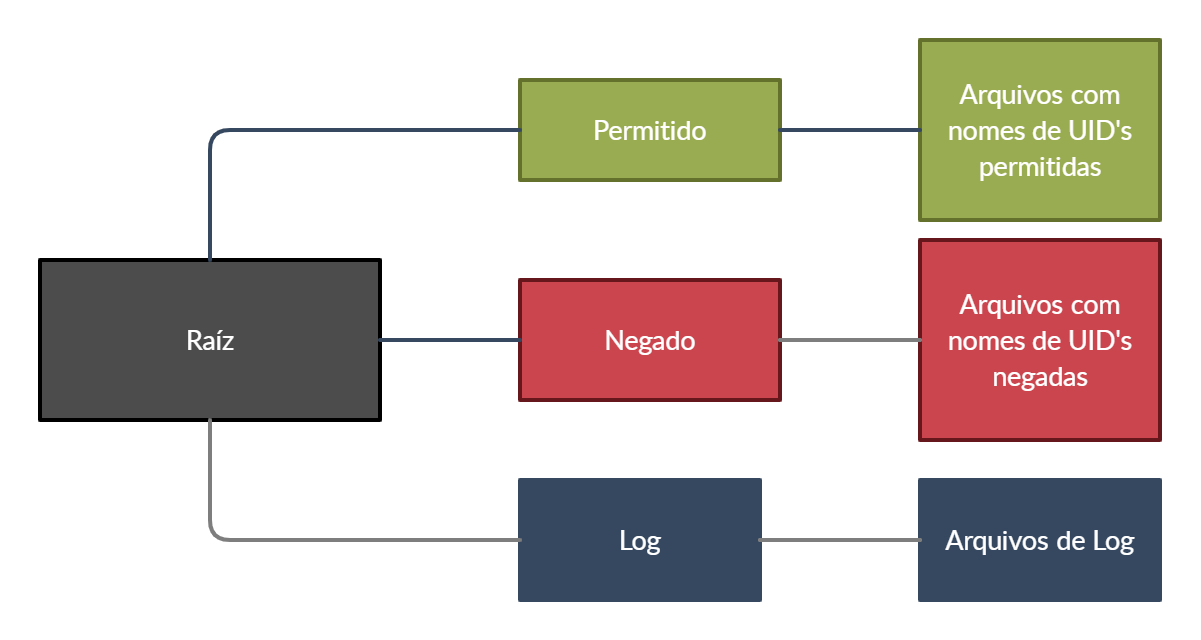
\includegraphics[scale=.3]{imagens/arvore}
	\\\textbf{Fonte:} Elaborado pelos autores
	\label{fig:arvore}
\end{figure}
\FloatBarrier

Parga adicionar o microSD ao circuito, precisamos de um socket
para este tipo de cartão (Figura ~\ref{fig:socket}). O socket será o intermediário entre
o cartão e o ATMEGA328p. A comunicação entre este socket também
é feita utilizando o protocolo ISP, assim, é necessário conectá-lo
utilizando quase o mesmo esquema utilizado para o sensor. A tabela
~\ref{tab:socketpinout} mostra as conexões necessáiras.

\FloatBarrier
\begin{figure}[!htbp]
	\centering
	\caption{Socket para cartão microSD}
	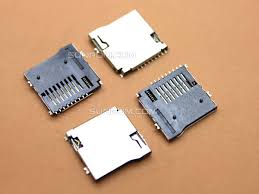
\includegraphics[scale=.5]{imagens/socket}
	\\\textbf{Fonte:} \href{https://www.sunrom.com/p/micro-sd-memory-card-socket}{Sunrom}
	\label{fig:socket}
\end{figure}
\FloatBarrier

\FloatBarrier
\begin{table}[!htbp]
	\centering
	\caption{Conexões do socket}
	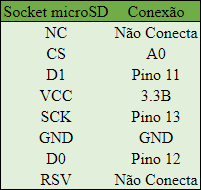
\includegraphics[scale=.7]{imagens/microsdpinout}
	\\ \vspace{0.2cm}
	\textbf{Fonte:} Elaborada pelos autores
	\label{tab:socketpinout}
\end{table}
\FloatBarrier

Como precisamos utilizar alguns pinos do arduino tanto
para o sensor quanto para o socket, precisaremos ligar
os dois em paralelo, além disso, precisamos adicionar
resistores de pull-up no CS do socket e no NSS do sensor.
Pro fim, é necessário ligar resistores de $10K\Omega$
no fio de MISO e D0, conectando-os no GND e 3.3V \cite{paul2014}. Assim,
a figura ~\ref{fig:esquemasd} mostra o circuito com o microSD.

\FloatBarrier
\begin{figure}[!htbp]
	\centering
	\caption{Esquema com cartão microSD}
	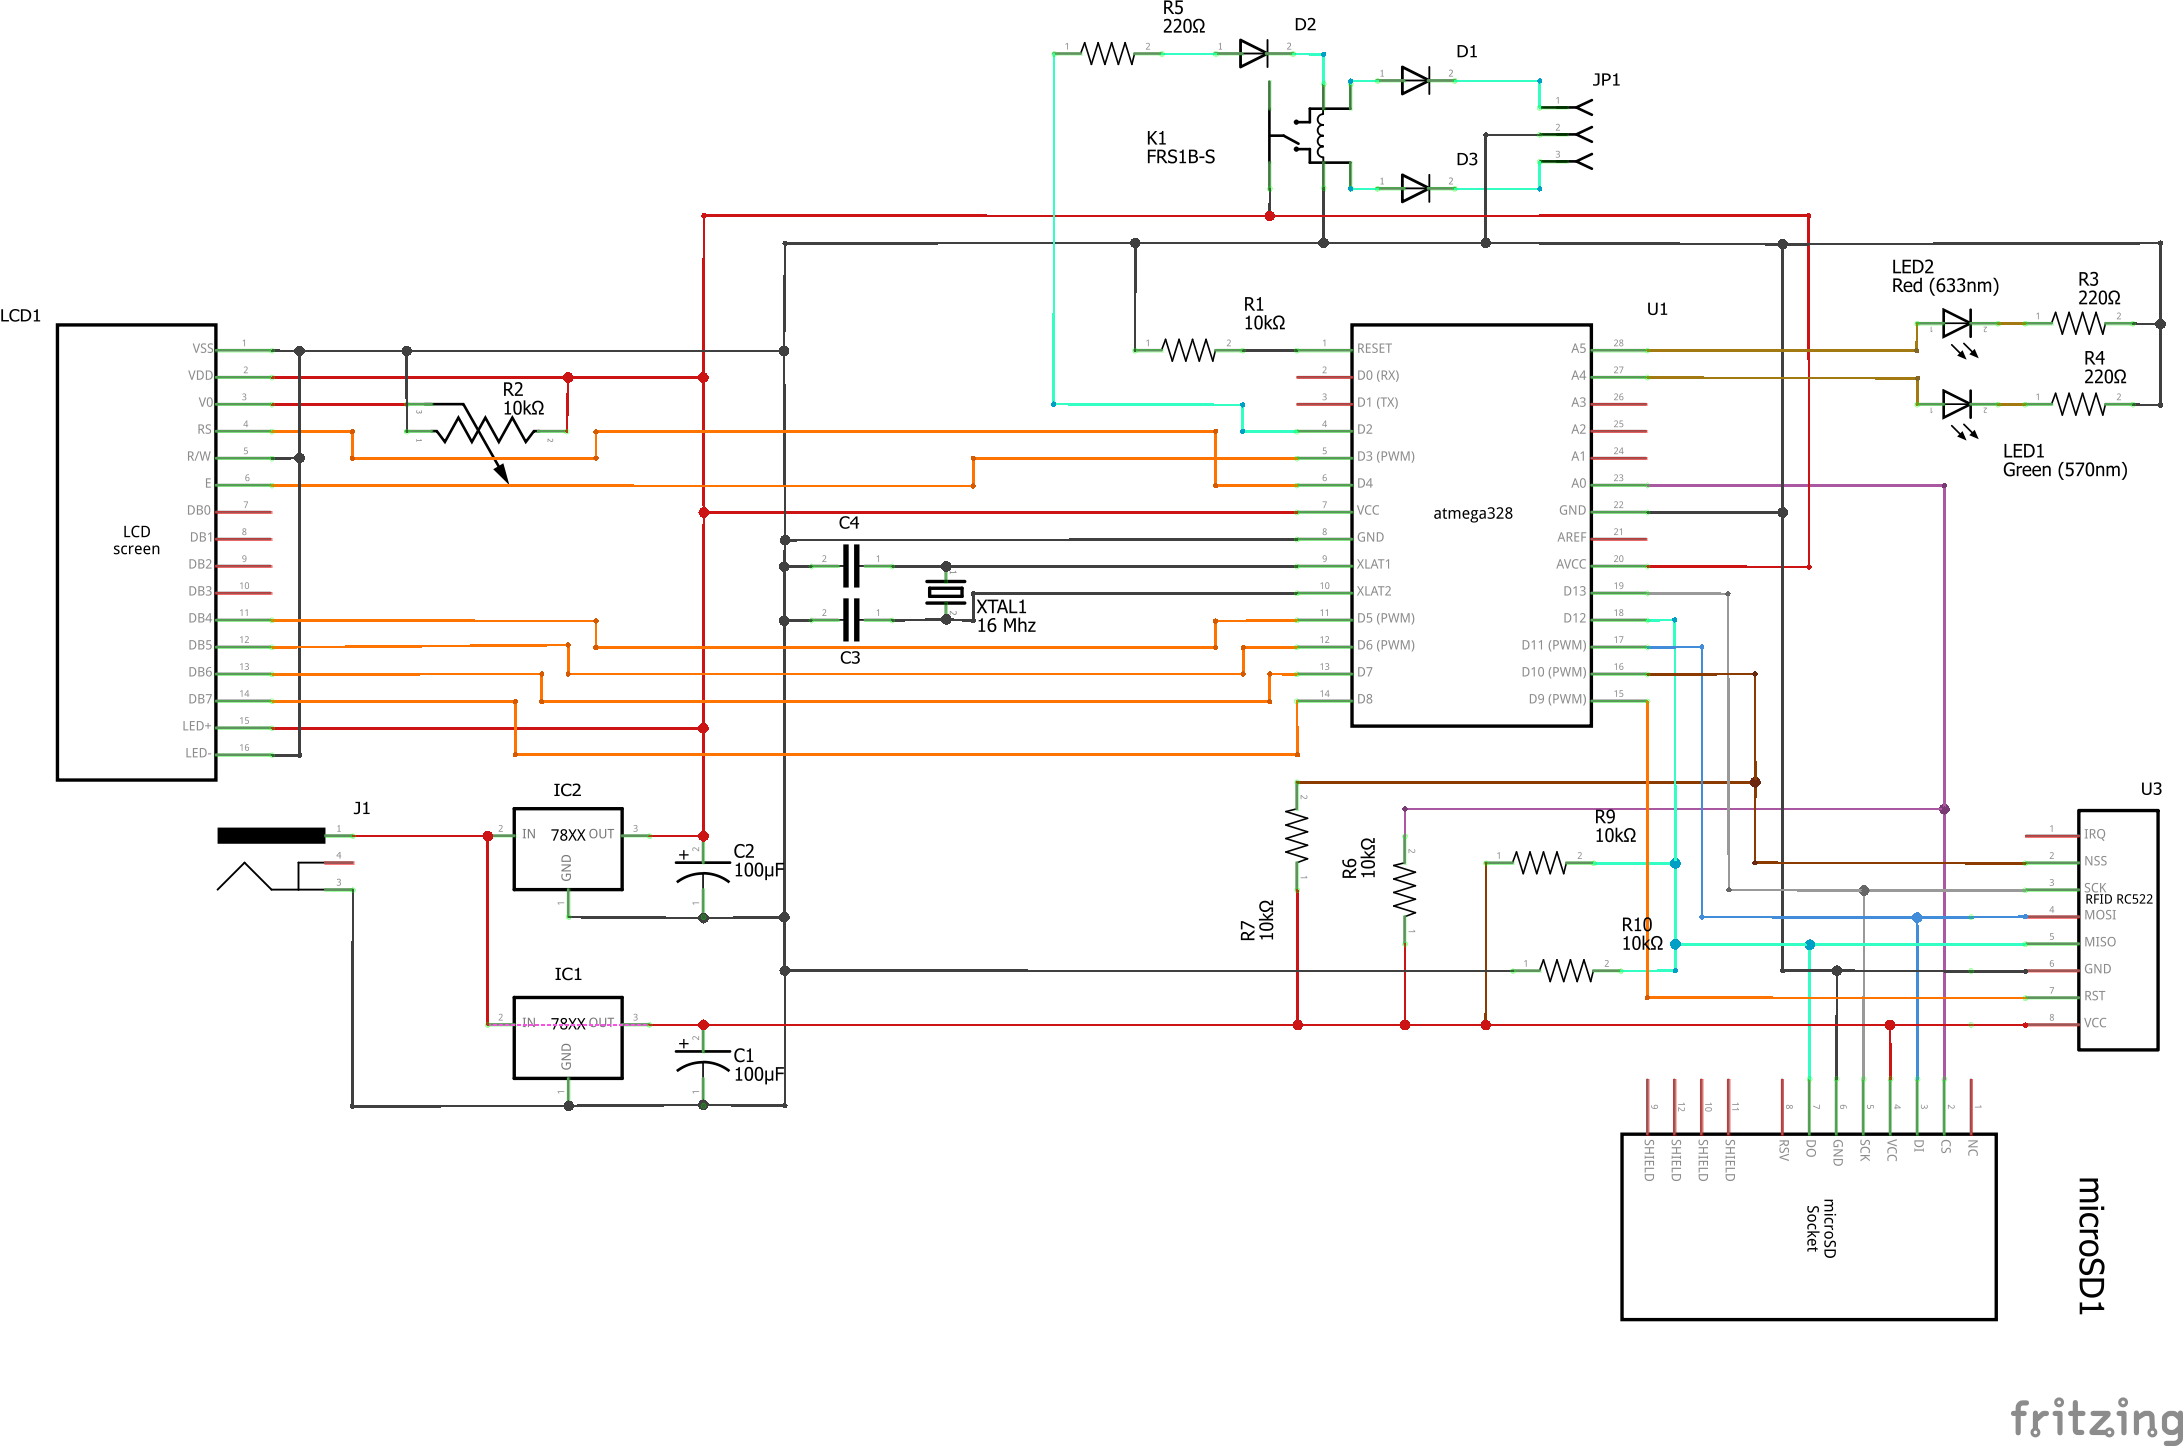
\includegraphics[scale=.7]{imagens/esquemasd}
	\\\textbf{Fonte:} Elaborada pelos autores
	\label{fig:esquemasd}
\end{figure}
\FloatBarrier

\section{Módulo RTC}
Um módulo RTC (Real-Time Clock) é um componente eletrônico
capaz de armazenar informações de tempo. No nosso projeto
optamos por utilizar o RTCDS3231.

Esse módulo se comunica com o ATMEGA328p por meio do protocolo I2C,
assim, precisamos de apenas 2 pinos analógicos, além de sua alimentação
\cite{mallari2020}. Suas conexões estão na tabela ~\ref{tab:dspinout}.

\FloatBarrier
\begin{table}[!htbp]
	\centering
	\caption{Conexões do módulo RTC DS3231}
	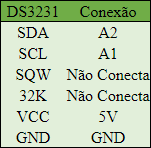
\includegraphics[scale=1]{imagens/dspinout}
	\\ \vspace{0.2cm}
	\textbf{Fonte:} Elaborada pelos autores
	\label{tab:dspinout}
\end{table}
\FloatBarrier

Colocando este módulo no circuito, chegamos ao esquema
da figura ~\ref{fig:final}. Além disso, o apêndice
~\ref{appendix:C} contém o código finalizado.

\FloatBarrier
\begin{figure}[!htbp]
	\centering
	\caption{Esquema finalizado do projeto}
	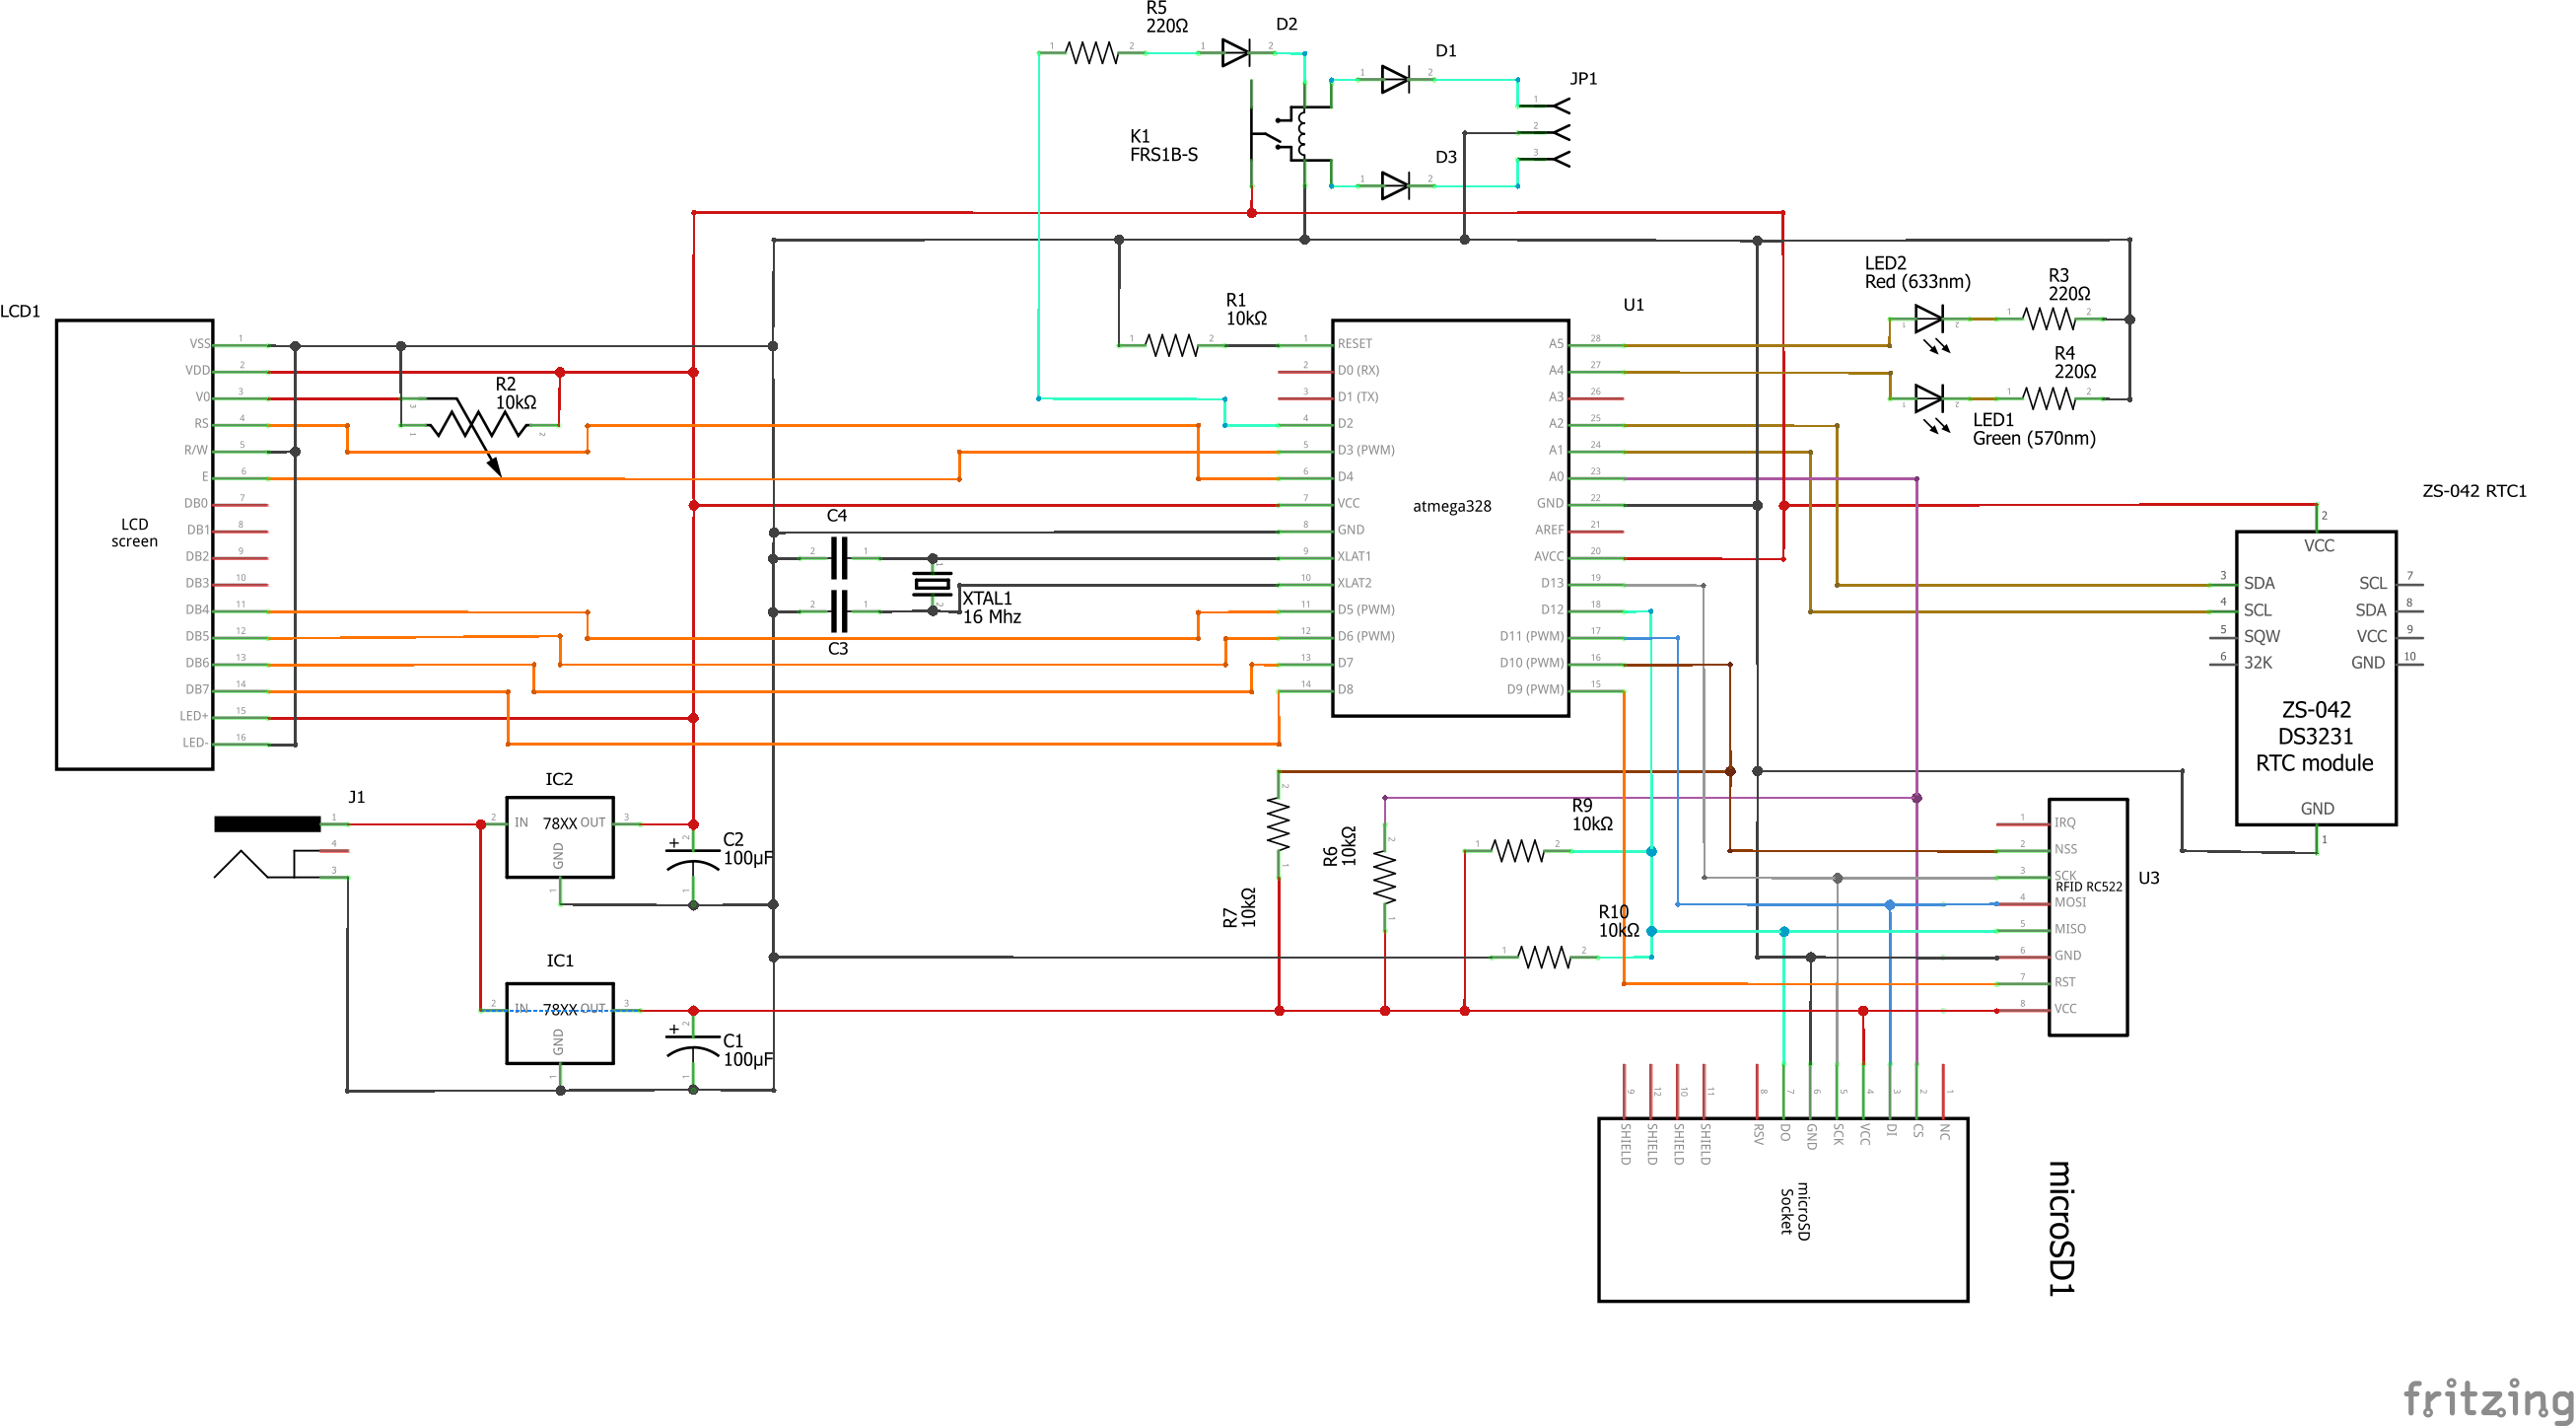
\includegraphics[scale=.7]{imagens/esquemalog}
	\\\textbf{Fonte:} Produzida pelos autores.
	\label{fig:final}
\end{figure}
\FloatBarrier